\chapter{Úvod do problematiky}

\indent

V první kapitole bychom se měli seznámit s pojmem Ultimate Frisbee. Dále pak nastíníme
problematiku pořádání turnajů v tomto minoritním sportu.

\section{Co je to Ultimate Frisbee}

\indent

Ultimate Frisbee je mladý a dynamicky se rozvíjející sport s létajícím talířem,
který se hraje od roku 1968 \cite{cald-ultimate}. Hraje jej přibližně sedm miliónů
hráčů ve více než 80 zemích světa a jeho popularita rok od roku stoupá \cite{usa-ultimate}.
Během posledních několika let je například běžné sledovat živé přenosy na sportovním kanálu ESPN
z Amerických soutěží, především profesionální ligy AUDL. Ultimate v roce 2015 dokonce získalo
uznání od Mezinárodního olympijského výboru \cite{cald-uznani}. Nejčastěji se hraje v kategoriích
open (muži), ženy, mix (smíšené týmy mužů a žen), junioři (do 19 let) a masters (nad 33 let).

\subsection{Pravidla}

\indent

Popularitě přidává fakt, že jde o celkem vzato nenáročnou hru na vybavení s jednoduchými pravidly:

\begin{quote}
Ultimate je kolektivní bezkontaktní sport, v němž vítězí tým, který má na konci hrací doby
vyšší počet bodů. Hraje se na hřišti o rozměrech cca 100x37 metrů (délka fotbalového hřiště,
polovina jeho šířky). Na obou koncích hřiště jsou vyznačeny koncové zóny o hloubce cca 18 metrů.

V ultimate proti sobě hrají dva sedmičlenné týmy. Smyslem hry je pomocí přihrávek dopravit disk
do soupeřovy koncové zóny a jeho chycením v zóně získat bod. Po chycení disku se hráč musí
zastavit a do 10 vteřin disk přihrát spoluhráči. Povoleným pohybem hráče s diskem je pivotování,
tedy otáčení se kolem vlastní osy s jednou nohou pevně na zemi. V ultimate hráči často střídají
útok a obranu při ztrátě disku, ke které dochází záhozem disku do autu, na zem, jeho zachycením
soupeřem nebo při dlouhém držení disku. Není povolen fyzický kontakt mezi hráči ani přetahování
o disk (\cite{cald-ultimate}).
\end{quote}

\begin{figure}[ht!]
\centering
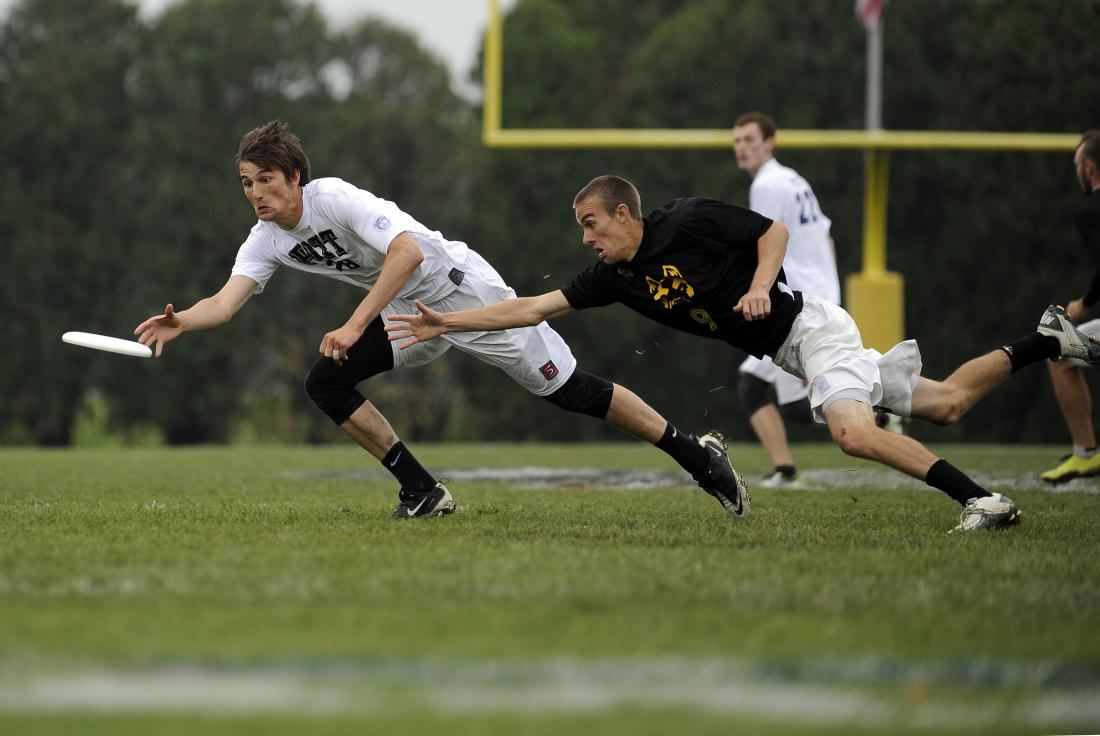
\includegraphics[width=130mm]{./images/ultimate-frisbee.jpg}
\caption{Fotografie z amerického časopisu TIME ze zápasu mezi univerzitními týmy z Pittsburgu a Floridy \cite{ultimate-time}.\label{overflow}}
\end{figure}


\subsection{Spirit of the Game}

\indent

Už od počátku je Ultimate Frisbee založeno na sportovním duchu, který klade odpovědnost
za fair play na samotné hráče. Předpokládá se vysoce soutěživá hra, ne však za cenu ztráty
vzájemné ohleduplnosti a vytracení radosti ze hry. Všechny přetupky na hřišti i mimo něj jsou
řešeny samotnými hráči. Jako jediná sportovní hra se tak obejde bez rozhodčích, a to i
na nejvyšších soutěžích, kterými jsou mistrovství Evropy a světa.

\medskip

Hraní fairplay je otázka cti. Na každém turnaji je vyhlašována cena Spirit of the Game,
která je cenou pro ty, kteří se chovali nejčestněji. Po každém zápase se týmy navzájem ohodnotí
v podobě číselného hodnocení a cenu pak získá tým s nejvyšším průměrem. Cena Spirit of the Game
je ceněna obdobně jako 1. místo.

\subsection{Ultimate v České republice}

\indent

V České republice zastřešuje sporty s létajícím talířem již od roku 1991\cite{cald-historie} Česká asociace
lé\-ta\-jícícho disku (dále jen ``ČALD''). V celé republice eviduje desítky zaregistrovaných
klubů (často zvaných oddílů), které se mezi sebou utkávají v rámci celého roku na akcích zvané turnaje.
Jenom za loňský rok jich bylo na našem území přes třicet \cite{cald-kalendar}.

\medskip

Většina turnajů nebo mistrovství pak trvá zpravidla více dnů, během kterých se odehrají desítky
utkání. A s přibývajícím počtem hráčů a fanoušků vzniká čím dál větší poptávka po online
přenosech a statistikách z těchto akcí.

% TODO: Bude potreba doplnit, protoze se jedna o dulezity pojem, ktery bude pak zpracovan.

%\subsection{Jak probíhá typický turnaj - IDEA - nedokonceno}

%\indent

%Několik dní před turnajem se zveřejní rozpis, zpravidla v podobě dokumentu na Google Drive apod.
%Ten je pak během turnajem editovaný a slouží jako jediný zdroj výsledků, který ... 

%Nejdůležitejším údajem jsou výsledky z jednotlivých zápasů. Ty jsou nejčastěji zapisovány
%na papír, který je vystaven na viditelném místě, aby si jej mohlo prohlédnout co nejvíce lidí.

%\medskip

%Částečně tyto procesy nahrazuje mobilní aplikace Catcher, ke které se ještě dostaneme.

% Vsechno se doposud pise na papir a je to proste cely na prd.
% TODO: Kdo vsechno, kolik lidi, na turnaji pobyva. Kolik probiha zapasu, treba i paralelne, kdo se o nej stara (navrh ma mobilni app). Co vsechno se da vycist z vysledku.
% TODO: Jeste doplnit dal.

% TODO: sem prijde rest api